
\begin{figure*}[h]
    \centering
    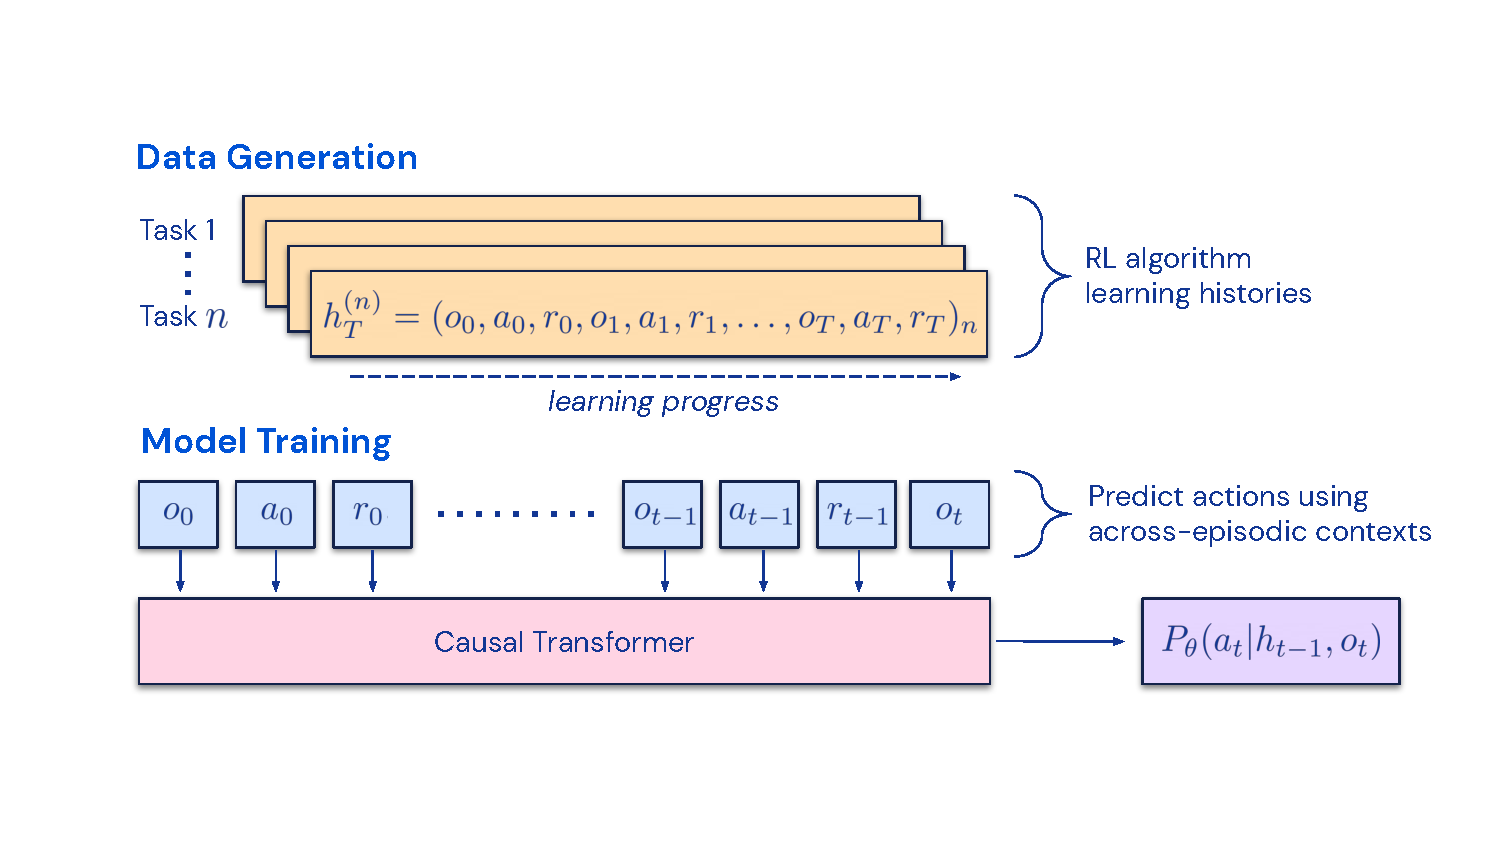
\includegraphics[width=\textwidth]{assets/images/main_fig_v5.pdf}
      \caption{\small \namedef has two steps -- (i) a dataset of learning histories is collected from individual single-task RL algorithms solving different tasks; (ii) a causal transformer predicts actions from these histories using across-episodic contexts. Since the RL policy improves throughout the learning histories, by predicting actions accurately \name learns to output an improved policy relative to the one seen in its context. \name models state-action-reward tokens, and does not  condition on returns. \looseness=-1}
  \label{fig:main}
\end{figure*}

\section{Introduction}
\label{sec:Introduction}

Transformers have emerged as powerful neural network architectures for sequence modeling \citep{vaswani2017attention}. A striking property of pre-trained transformers is their ability to adapt to downstream tasks through prompt conditioning or in-context learning.
After pre-training on large offline datasets, large transformers have been shown to generalize to downstream tasks in text completion~\citep{brown2020gpt3}, language understanding~\citep{devlin2018bert}, and image generation~\citep{yu2022parti}.

Recent work demonstrated that transformers can also learn policies from offline data by treating offline Reinforcement Learning (RL) as a sequential prediction problem. While~\citet{chen2021dt} showed that transformers can learn single-task policies from offline RL data via imitation learning, subsequent work showed that transformers can also extract multi-task policies in both same-domain~\citep{lee2022mgdt} and cross-domain settings~\citep{reed2022gato}. These works suggest a promising paradigm for extracting generalist multi-task policies – first collect a large and diverse dataset of environment interactions, then extract a policy from the data via sequential modeling. We refer to the family of approaches that learns policies from offline RL data via imitation learning as Offline Policy Distillation, or simply Policy Distillation\footnote{What we refer to as Policy Distillation is similar to~\citet{rusu16pd} but the policy is distilled from offline data, not a teacher network.} (PD). 


Despite its simplicity and scalability, a substantial drawback of PD is that the resulting policy does not improve incrementally from additional interaction with the environment. For instance, the Multi-Game Decision Transformer~\citep[MGDT,][]{lee2022mgdt} learns a return-conditioned policy that plays many Atari games while Gato~\citep{reed2022gato} learns a policy that  solves tasks across diverse environments by inferring tasks through context, but neither method can improve its policy in-context through trial and error. MGDT adapts the transformer to new tasks by finetuning the model weights while Gato requires prompting with an expert demonstration to adapt to a new task. In short, Policy Distillation methods learn policies but not Reinforcement Learning algorithms.

We hypothesize that the reason Policy Distillation does not improve through trial an error is that it trains on data that does not show learning progress. Current methods either learn policies from data that contains no learning ({\it e.g.} by distilling fixed expert policies) or data with learning ({\it e.g.} the replay buffer of an RL agent) but with a context size that is too small to capture policy improvement.

Our key observation is that the sequential nature of learning within RL algorithm training could, in principle, make it possible to model the process of reinforcement learning itself as a causal sequence prediction problem.
Specifically, if a transformer’s context is long enough to include policy improvement due to learning updates it should be able to represent not only a fixed policy but a policy improvement operator by attending to states, actions and rewards from previous episodes.
This opens the possibility that any RL algorithm can be distilled into a sufficiently powerful sequence model such as a transformer via imitation learning, converting it into an in-context RL algorithm.

We present \namedefnospace, a method that learns an in-context policy improvement operator by optimizing a causal sequence prediction loss on the learning histories of an RL algorithm.
\name has two components. First, a large multi-task dataset is generated by saving the training histories of an RL algorithm on many individual tasks. Next, a transformer models actions causally using the preceding learning history as its context. Since the policy improves throughout the course of training of the source RL algorithm, \name is forced to learn the improvement operator in order to accurately model the actions at any given point in the training history. Crucially, the transformer context size must be sufficiently large (\ie \, across-episodic) to capture improvement in the training data. The full method is shown in Fig.~\ref{fig:main}. 

We show that by imitating gradient-based RL algorithms using a causal transformer with sufficiently large contexts, \name can reinforcement learn new tasks entirely in-context. We evaluate \name across a number of partially observed environments that require exploration, including the pixel-based Watermaze~\citep{morris1981watermaze} from DMLab~\citep{beattie2016dmlab}. We show that AD is capable of in-context exploration, temporal credit assignment, and generalization. We also show that AD learns a more data-efficient algorithm than the one that generated the source data for transformer training.
To the best of our knowledge, AD is the first method to demonstrate in-context reinforcement learning via sequential modeling of offline data with an imitation loss.
